% !TEX encoding = UTF-8 Unicode

Em um primeiro momento, foi definida uma linguagem de programação e identificados os tipos de átomos. Para cada átomo foi escrito uma gramática linear representativa da sua lei de formação e um reconhecedor para o átomo. Desse modo, as gramáticas assim escritas foram unidas e convertidas em um autômato finito, o qual foi transformado em um transdutor e implementado como sub-rotina, dando origem ao analisador léxico propriamente dito.

Também foi criada uma função principal para chamar o analisador léxico e possibilitar o seu teste. Cabe ressaltar que foi utilizado o analisador léxico do trabalho como base para esse, visto que a estrutura e alguns \emph{tokens} eram os mesmos. Algumas das alterações feitas para adaptar o transdutor foram:

\begin{itemize}
	\item \textbf{IDENT vs PRED + INF}: Antes, só havíamos um \emph{token} para representar identificadores de alguma forma, chamados de \textbf{IDENT}. Porém, ao observar a sintaxe do \emph{SimpPro}, foi necessário alterar o léxico para diferenciar tokens que começam com minúscula (chamado \textbf{PRED}) ou maiúscula (chamado \textbf{INF});
	\item Os operadores específicos dessa linguagem como :- e ?- foram considerados novas classes de \emph{tokens}, para facilitar a sua identificação.
\end{itemize} 

A Figura~\ref{fig:transdutor} representa o transdutor utilizado para reconhecer os \emph{tokens} da linguagem.

\begin{figure}[htbp]
    \centering
    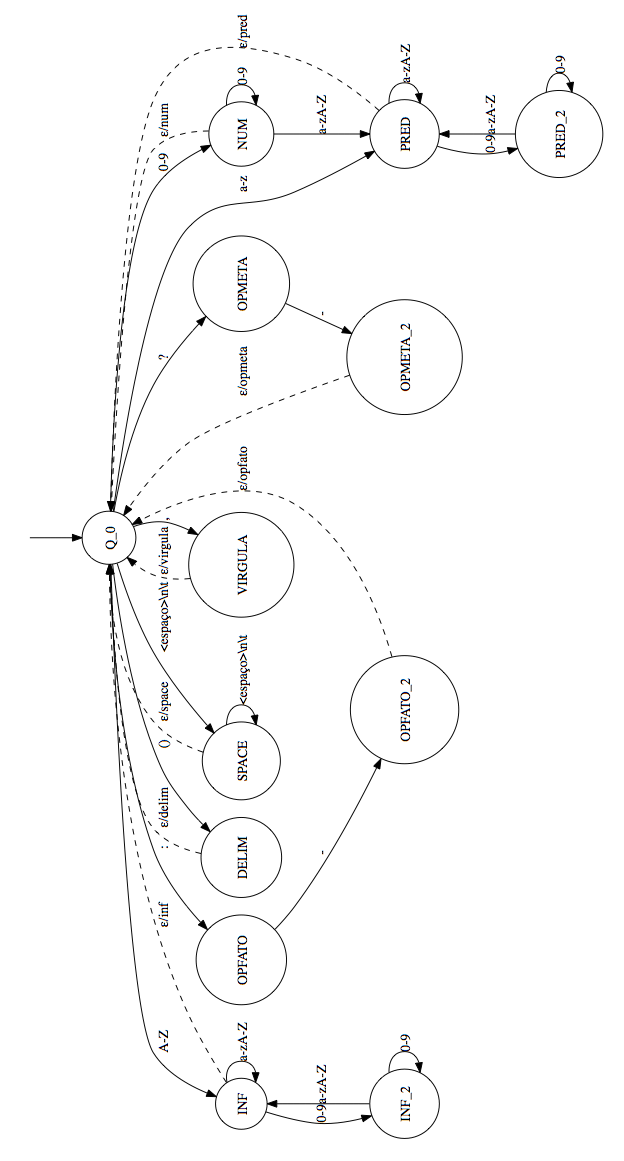
\includegraphics[width=0.7\textwidth]{./images/transdutor.png}
    \caption{Transdutor desenvolvido}
    \label{fig:transdutor}
\end{figure}
